\documentclass{article}

\usepackage{geometry}
\usepackage{fancyhdr}
\usepackage{amsmath, amssymb}
\usepackage{graphicx}
\usepackage{color}
\definecolor{bg}{rgb}{0.89, 0.95, 0.71} % background e3f3b4
\definecolor{ac}{rgb}{0.50, 0.18, 0.41} % accent c491b6
\definecolor{rc}{rgb}{0.77, 0.57, 0.71} % rule 7f2f69
\usepackage{listings}
\lstset{
       basicstyle=\small\ttfamily,
       xleftmargin=1em,
       }
\lstdefinestyle{latex}{language=TeX,
                       backgroundcolor=\color{bg},
                       basicstyle=\small\ttfamily,
                       frame=leftline,
                       xleftmargin=1.4em, 
                       framexleftmargin=.8em}
\lstdefinestyle{cmdline}{
                         }
\usepackage{url}
\usepackage[pdftex, 
            bookmarks, 
            colorlinks=true,
            linkcolor=black, 
            plainpages = false,
            pdfpagemode = UseNone,
            pdfstartview = FitH, 
            citecolor = ac, urlcolor = ac, filecolor = ac]{hyperref}

\usepackage[para]{footmisc}
% Change horiz room between fn mark and fn hskip from .5em 
% Suggested to RF making this settable
\makeatletter
\long\def\@makefntext#1{\leavevmode
\@makefnmark\nobreak
\hskip.05em\relax#1%
}
\makeatother
%\newcommand{\texdoc}[1]{\/\footnote{\protect\texttt{#1}}}
\newcommand{\citelink}[3]{\href{#1}{#2}~\cite{#3}}
\newcommand{\bibliolink}[2]{\href{#1}{\nolinkurl{#1}}, \href{#1}{#2}}

\setlength{\parskip}{0.75ex}
\makeatletter % from emma pease at csli.stanford.edu
% \@startsection {NAME}{LEVEL}{INDENT}{BEFORESKIP}{AFTERSKIP}{STYLE} 
%            optional * [ALTHEADING]{HEADING}
%    Generic command to start a section.  
%    NAME       : e.g., 'subsection'
%    LEVEL      : a number, denoting depth of section -- e.g., chapter=1,
%                 section = 2, etc.  A section number will be printed if
%                 and only if LEVEL < or = the value of the secnumdepth
%                 counter.
%    INDENT     : Indentation of heading from left margin
%    BEFORESKIP : Absolute value = skip to leave above the heading.  
%                 If negative, then paragraph indent of text following 
%                 heading is suppressed.
%    AFTERSKIP  : if positive, then skip to leave below heading,
%                       else - skip to leave to right of run-in heading.
%    STYLE      : commands to set style
%  If '*' missing, then increments the counter.  If it is present, then
%  there should be no [ALTHEADING] argument.  A sectioning command
%  is normally defined to \@startsection + its first six arguments.
\def\section{\@startsection {section}{1}{\z@}{2.5ex plus .6ex minus 
    .2ex}{1.0ex plus .15ex}{\hspace*{-3em}\Large\bf\color{ac}}}
\def\subsection{\@startsection{subsection}{2}{\z@}{1.5ex plus .3ex minus 
   .1ex}{.2ex plus .1ex}{\hspace*{-3em}\bf\large\color{ac}}}
\makeatother
\setcounter{secnumdepth}{0}

\newlength{\rulelength}
\setlength{\rulelength}{\linewidth}
\addtolength{\rulelength}{9.5em}
\title{Getting something out of \LaTeX{}}
\author{Jim Hef{}feron}

\pagestyle{plain}
\begin{document}
\thispagestyle{empty}
% \maketitle
\setlength{\unitlength}{1in}
\begin{picture}(0,0)(0,0)
  \put(-0.5,-.84){\mbox{\color{bg}\rule{2.32in}{1.15in}}}
\end{picture}
\makeatletter
\vspace*{3ex}
\par\noindent{\hspace*{-1.5em}\LARGE\bf \@title}
\vspace*{-1.2ex}
\par\noindent{\textcolor{rc}{\hspace*{-1.5em}\rule{\rulelength}{1.05pt}}}
\vspace*{-.5ex}
\par\noindent{\hspace*{-1.5em}\large \@author}
\vspace*{5ex}
\makeatother

This is for people considering using \LaTeX{}.
This is not a tutorial.
Instead, 
it takes you through making a first document.
If this quick taste leaves you wanting more
then you are ready to go through a tutorial.

Because this is a just a taste, we will skip many things.
And, for those things that we will discuss, 
we will see only one way to do them.
For instance, in the first section there are a number of ways to get 
the software but we will just name one.
This approach has the disadvantage of leaving you without a full understanding
of the system 
but has the advantage that in a couple of hours 
you will know whether
\LaTeX{} is a tool that can help you.

  



\section{Get the software}

\LaTeX{} is how we will use the \TeX{} suite of 
programs.
So you must download that suite, if you don't already have it.
We will describe only options that are free.

If your computer system is Windows then download 
\citelink{http://www.miktex.org}{MiK\TeX}{miktex}.\footnote{For people with a printed version of this document we list links at the end.}
If you have a Unix-like system such as GNU/Linux then get
\citelink{http://www.tug.org/texlive/}{\TeX{} Live}{texlive}.
For a Macintosh get
\citelink{http://www.tug.org/mactex/}{Mac\TeX}{mactex},
a version of \TeX{}~Live with some Mac-specific add-ons.

All three downloads are big but all three install easily (of course,
you must carefully follow the directions; in particular on 
a Unix-like system you will need to alter your \texttt{PATH}).
Here we are only giving \LaTeX{} a try so we will skip most things.




\subsection{Use an editor}

We don't write \LaTeX{} with a word processor.
A word processor combines many of the jobs that must be done to 
produce a document, such as entering and moving the text, formatting it
into paragraphs, producing a PDF file, etc.
In a \TeX{}-based system those jobs are done separately.

Instead, we write \LaTeX{} with an editor, 
a program that is specialized at moving text around in a computer file.
There are many editors,
including some specifically for writing \LaTeX{}, but below
our documents are small so any editor will do. 
Just to name a couple of names:
on a Windows system you can use Notepad,
while on a Unix-like system or a Mac you can use Emacs.





\section{Get it to work}

Having picked an editor, you can write a first document.
Make a new directory
named \nolinkurl{latex-first}  
(your system might use the term ``folder'').
Open a terminal window and in that window, change into that directory
(possibly you would use the command \verb!cd latex-first!).

Next start your editor.
Open the new file
\nolinkurl{latex-first.tex}
in the \nolinkurl{latex-first} directory. 
Enter the text below, line for line, as it is written
(without spaces on the left margin).
\begin{lstlisting}[style=latex]
\documentclass{article}
\usepackage{geometry}
\usepackage{fancyhdr}
\usepackage{amsmath,amsthm,amssymb}
\usepackage{graphicx}
\usepackage{hyperref}

\begin{document}
Hello world!
\end{document}
\end{lstlisting}
Many of those things are boilerplate~--- lines that I put into every
\LaTeX{} file.
We'll ignore what they mean for a while to focus on getting
out a first document.

Save that file.
Go back to your terminal window and enter this command.
\begin{lstlisting}
pdflatex latex-first
\end{lstlisting}
If that worked then you should see perhaps forty lines of text, 
starting with something like 
\begin{lstlisting}
This is pdfTeXk, Version 3.1415926-1.40.9 (Web2C 7.5.7)
 %&-line parsing enabled.
entering extended mode
\end{lstlisting}
and ending with something like this.
\begin{lstlisting}
Output written on latex-first.pdf (1 page, 6195 bytes).
Transcript written on latex-first.log.
\end{lstlisting}
If you had errors, see the subsection below.

You can view the output file \nolinkurl{latex-first.pdf} with
whatever program your system uses to view PDF.
\begin{center}
  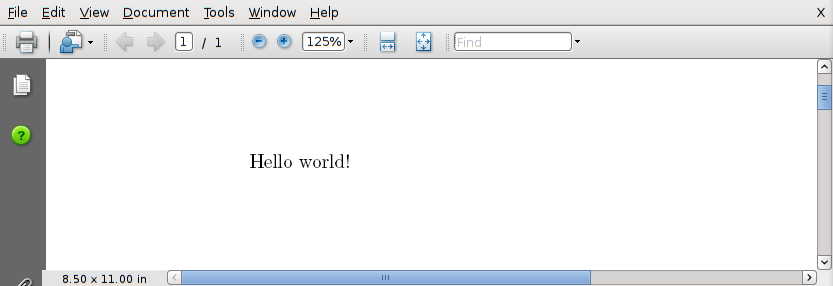
\includegraphics[scale=.35]{latex-first.png}
\end{center}

\subsection{Handle errors}

Check that you have typed the lines exactly.
Some seemingly small typing changes give large changes in the
result, including causing a document to not work.
So that you can be sure there isn't a typing discrepancy, 
you can get a known-good copy of
\nolinkurl{latex-first.tex}; see 
\protect\citelink{http://www.ctan.org/tex-archive/info/first-latex-doc/}{this document's source}{firstdoc}.

If your run ends with a question mark, then you can type `\verb!x!' and
hit the `Enter' key to get out.

\LaTeX's error messages can be hard to understand.
If you know someone with some experience, of course that's great.
If not, I've had good luck with putting the error message into a 
search engine.






\section{Get more out}

The first document is short so that it has fewer parts to go wrong.
But we've already seen some basics.
The file you type mixes text and commands.
The commands for \LaTeX{}, such as \verb!\begin{document}!,
start with a backslash
and sometimes have arguments contained in curly braces
(or, we'll see below, sometimes square brackets).

The document we've made starts out with margins, typeface, etc., specified 
in the class \verb!article!.
We've modified the behavior in small ways by bringing in some
packages such as \verb!graphicx!, which will allow us to include
graphic files.
 
Next
we'll make a longer and more complex document.
Start the same way:
make a new directory
named \nolinkurl{latex-second},
open a terminal window, and change into the new directory.
Then move back to your editor window and
open a new file
\nolinkurl{latex-second.tex}
in the \nolinkurl{latex-second} directory. 
Enter this.
\begin{lstlisting}[style=latex]
\documentclass{article}
\usepackage{geometry}
\usepackage{fancyhdr}
\usepackage{amsmath,amsthm,amssymb}
\usepackage{graphicx}
\usepackage{hyperref}
\usepackage{lipsum}

\begin{document}
This is some preamble text that you enter yourself.

Below is a command that will automatically generate seven paragraphs
of text that is commonly used for examples in this field.

\lipsum[1-7]
\end{document}
\end{lstlisting}
Save that file and in the terminal window run
\verb!pdflatex latex-second!.
Your system's PDF reader should show this.
\begin{center}
  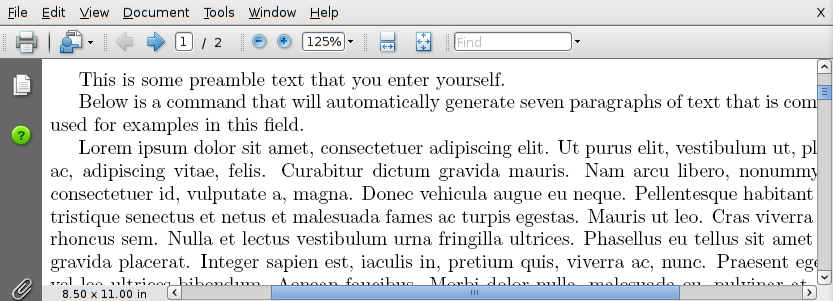
\includegraphics[scale=.35]{latex-second-a.png}
\end{center}

If you have used a word processor then you will have noticed the 
difference between that tool and \LaTeX{}.
A word processor moves the text around as you type it.
With \LaTeX{}, you describe what you want and then it goes off and 
figures out how best to do that.
For instance, below we will
tell \LaTeX{} to make a section and the system 
handles the font changes, vertical space, etc.

In your editor, change the file \nolinkurl{latex-second.tex} to say this.
\begin{lstlisting}[style=latex]
\documentclass{article}
\usepackage{geometry}
\usepackage{fancyhdr}
\usepackage{amsmath,amsthm,amssymb}
\usepackage{graphicx}
\usepackage{hyperref}
\usepackage{lipsum}

\begin{document}
This is some preamble text that you enter yourself.

\section{Text for the first section}
\lipsum[1]

\subsection{Text for a subsection of the first section}
\lipsum[2-3]

\subsection{Another subsection of the first section}
\lipsum[4-5]

\section{The second section}
\lipsum[6]

\subsection{Title of the first subsection of the second section}
\lipsum[7]
\end{document}
\end{lstlisting}
Here is the resulting output.
\begin{center}
  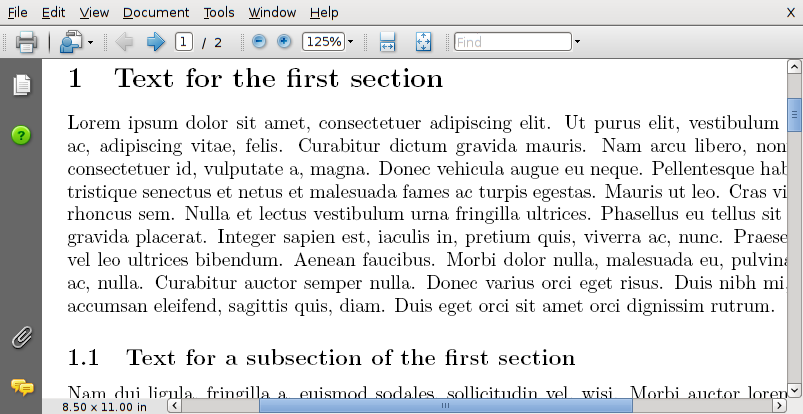
\includegraphics[scale=.35]{latex-second-b.png}
\end{center}
Note that numbering of the sections and subsections is done automatically.
How to change how they look is beyond this document, but the point is that
the system generates those for you.

With those, we can illustrate cross-references.
Change the document's text to this.
\begin{lstlisting}[style=latex]
\begin{document}
This is some preamble text that you enter yourself.

\section{Text for the first section}
\lipsum[1]

\subsection{Text for a subsection of the first section}
\lipsum[2-3]
\label{labelone}

\subsection{Another subsection of the first section}
\lipsum[4-5]
\label{labeltwo}

\section{The second section}
\lipsum[6]

Refer again to \ref{labelone}.
Note also the discussion on page \pageref{labeltwo}

\subsection{Title of the first subsection of the second section}
\lipsum[7]
\end{document}
\end{lstlisting}
Run 
\verb!pdflatex latex-second!
and look at the PDF file.
Notice that the references that we just entered didn't work~--- they appear
as question marks.
As \LaTeX{} runs it saves labels to a file.
When you run a file with a first-time label it has not yet been saved.
The question marks go away when you run \verb!pdflatex latex-second! 
a second time.
\begin{center}
  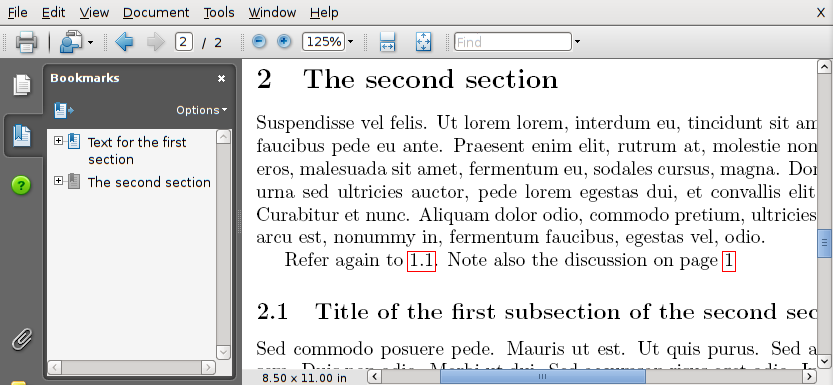
\includegraphics[scale=.35]{latex-second-c.png}
\end{center}
(When you are writing a real document, because you are fixing typos, etc.,
you will run \LaTeX{} a number of times, so in practice having to
rerun the command isn't an issue.)

We'll finish by adding footnotes, a
table of contents, and a bibliography.
Edit \nolinkurl{latex-second.tex} to say this. 
\begin{lstlisting}[style=latex]
\documentclass{article}
\usepackage{geometry}
\usepackage{fancyhdr}
\usepackage{amsmath,amsthm,amssymb}
\usepackage{graphicx}
\usepackage{hyperref}
\usepackage{lipsum}

\title{Test document}
\author{Your name \\ \url{you@example.com}}
\date{2009-Oct-12}
\begin{document}
\maketitle
\tableofcontents
\newpage

This is some preamble text that you enter 
yourself.\footnote{First footnote.}\footnote{Second footnote.}

\section{Text for the first section}
\lipsum[1]

\subsection{Text for a subsection of the first section}
\lipsum[2-3]
\label{labelone}

\subsection{Another subsection of the first section}
\lipsum[4-5]
\label{labeltwo}

\section{The second section}
\lipsum[6]

Refer again to \ref{labelone}.\cite{ConcreteMath}
Note also the discussion on page \pageref{labeltwo}

\subsection{Title of the first subsection of the second section}
\lipsum[7]

\begin{thebibliography}{9}
\bibitem{ConcreteMath}
Ronald L. Graham, Donald E. Knuth, and Oren Patashnik, 
\textit{Concrete Mathematics}, 
Addison-Wesley, Reading, MA, 1995.
\end{thebibliography}
\end{document}
\end{lstlisting}
Run \verb!pdflatex latex-second!  
(in the \verb!\begin{thebibliography}{9}! line, 
the \verb!9! tells \LaTeX{} that
the widest reference has one digit).  

Try changing the margins by altering the second
line to \verb!\usepackage[margin=1in]{geometry}!.
You can also experiment with the headings by changing the \verb!fancyhdr! 
line to this.
\begin{lstlisting}[style=latex]
\usepackage{fancyhdr}
\pagestyle{fancy}
\lhead{\today}
\chead{}
\rhead{Test document}
\lfoot{}
\cfoot{\thepage}
\rfoot{}
\end{lstlisting}


\section{Get math}

Many people interested in \LaTeX{} 
want to include mathematics.
The examples below are from \textit{Concrete Mathematics}~\cite{ConcreteMath}.
(We'll stop giving the complete listings of the input files,
and we'll stop showing screenshots to instead just give the output directly.)

Add this text, for instance before the bibliography.
\begin{lstlisting}[style=latex]
There are $\binom{2n+1}{n}$ sequences with $n$ occurrences of 
$-1$ and $n+1$ occurrences of $+1$, and Raney's lemma
tells us that exactly $1/(2n+1)$ of these sequences have all
partial sums positive.
\end{lstlisting} % page 360
It produces this output.
\begin{center}
\begin{minipage}{0.8\textwidth}
There are $\binom{2n+1}{n}$ sequences with $n$ occurrences of 
$-1$ and $n+1$ occurrences of $+1$, and Raney's lemma
tells us that exactly $1/(2n+1)$ of these sequences have all
partial sums positive.
\end{minipage}
\end{center}
This input
\begin{lstlisting}[style=latex]
Elementary calculus suffices to evaluate $C$ if we are clever enough
to look at the double integral
\begin{equation*}
  C^2
  =\int_{-\infty}^{+\infty} e^{-x^2} \mathrm{d}x
   \int_{-\infty}^{+\infty} e^{-y^2} \mathrm{d}y\;.
\end{equation*}
\end{lstlisting} % page 485
gives this.
\begin{center}
\begin{minipage}{0.8\textwidth}
Elementary calculus suffices to evaluate $C$ if we are clever enough
to look at the double integral
\begin{equation*}
  C^2
  =\int_{-\infty}^{+\infty} e^{-x^2} \mathrm{d}x
   \int_{-\infty}^{+\infty} e^{-y^2} \mathrm{d}y\;.
\end{equation*}
\end{minipage}
\end{center}
And this source
\begin{lstlisting}[style=latex]
Solve the following recurrence for $n,k\geq 0$:
\begin{align*}
  Q_{n,0} &= 1
  \quad Q_{0,k} = [k=0];  \\
  Q_{n,k} &= Q_{n-1,k}+Q_{n-1,k-1}+\binom{n}{k}, \quad\text{for $n,k>0$.}
\end{align*}
\end{lstlisting} % page 250
produces this result.
\begin{center}
\begin{minipage}{0.8\textwidth}
Solve the following recurrence for $n,k\geq 0$:
\begin{align*}
  Q_{n,0} &= 1
  \quad Q_{0,k} = [k=0];  \\
  Q_{n,k} &= Q_{n-1,k}+Q_{n-1,k-1}+\binom{n}{k}, \quad\text{for $n,k>0$.}
\end{align*}
\end{minipage}
\end{center}
The \verb!\usepackage{ams...! line in our source files
allow us to use the American Math Society's packages.
For example, the \texttt{align*} above is available because we
used \texttt{amsmath}.

We also have access to the AMS's symbols. 
A simple example is that we can get $\mathbb{Z}$ with the command
\verb!$\mathbb{Z}$!.
One more example shows a long arrow, and some other useful commands
\begin{lstlisting}[style=latex]
Therefore
\begin{equation*}
a\equiv b\pmod{m}
\qquad\Longleftrightarrow\qquad
a\equiv b \pmod{p^{m_p}}\quad\text{for all $p$}  
\end{equation*}
if the prime factorization of $m$ is $\prod_p p^{m_p}$.
\end{lstlisting} % page 126 
that produce this.
\begin{center}
\begin{minipage}{0.8\textwidth}
Therefore
\begin{equation*}
a\equiv b\pmod{m}
\qquad\Longleftrightarrow\qquad
a\equiv b \pmod{p^{m_p}}\quad\text{for all $p$}  
\end{equation*}
if the prime factorization of $m$ is $\prod_p p^{m_p}$.
\end{minipage}
\end{center}
(The
\citelink{http://mirror.ctan.org/info/symbols/comprehensive/symbols-letter.pdf}{\textit{Comprehensive \LaTeX{} Symbols List}}{comprehensive} 
shows the widely-available symbols.)

The \verb!amsthm! package gives us access to theorem environments,
but those go beyond the scope of this document.



\section{Got it?}
You now have a feel for \LaTeX.
To go on, 
see the tutorial
\citelink{http://mirror.ctan.org/info/lshort}{\textit{The Not-So-Short Guide to \LaTeX  2e}}{notsoshort}
or the 
\citelink{http://www.tug.org.in/tutorials.html}{Indian \TeX{} Users Group's tutorial}{indian}.
More references are in the
\citelink{http://mirror.ctan.org/tex-archive/info/latex-doc-ptr/}{\LaTeX{} Document Pointer}{latexdocptr}.

If what you've seen seems very different from what you are used to,
and you'd like an overview of the advantages of \LaTeX{},
see
\citelink{http://www.tug.org/TUGboat/Articles/tb22-1-2/tb70heff.pdf}{Why \TeX?}{whytex}.

When you take up \LaTeX{} for real-life documents, you need
to choose a good editing program. 
In particular, people often use systems where the editor is integrated with
other components such as an output view, a spell checker that works
with \LaTeX{}, etc.
For advice, ask \LaTeX{} users that you know or click around on the Internet, 
for instance on
\citelink{http://groups.google.com/group/comp.text.tex/topics?gvc=2}{\url{comp.text.tex}}{ctt}.
(For what it is worth, I use \verb!emacs! with the AUC\TeX{} add-on.  
On the Macintosh, many people use
\citelink{http://www.uoregon.edu/~koch/texshop/}{\TeX{} Shop}{texshop}.
A cross-platform editor, developed for the \TeX{} Users Group
with the goal of simplicity, is 
\citelink{http://www.tug.org/texworks/}{\TeX{}works}{texworks}.)

% \raggedright
\begin{thebibliography}{99}
\bibitem{comprehensive}
\bibliolink{http://mirror.ctan.org/info/symbols/comprehensive/symbols-letter.pdf}{\textit{Comprehensive \LaTeX{} Symbols List}}, 
Scott Pakin, 
2008.

\bibitem{ConcreteMath}
\textit{Concrete Mathematics}, 
Ronald L. Graham, Donald E. Knuth, and Oren Patashnik, 
Addison-Wesley, Reading, MA, 1995.

\bibitem{ctt}
\bibliolink{http://groups.google.com/group/comp.text.tex/topics?gvc=2}{\url{comp.text.tex} usenet group},
group authorship, 
2009.

\bibitem{firstdoc}
\bibliolink{http://www.ctan.org/tex-archive/info/first-latex-doc/}{\textit{Getting something out of \LaTeX}} (source for this document), 
Jim Hefferon, 
2009.

\bibitem{indian}
\bibliolink{http://www.tug.org.in/tutorials.html}{Indian \TeX{} Users Group's tutorial}, 
Indian \TeX{} Users Group,
2003.

\bibitem{latexdocptr}
\bibliolink{http://mirror.ctan.org/tex-archive/info/latex-doc-ptr/}{\LaTeX{} Document Pointer}, 
Jim Hef{}feron, others,
2009.

\bibitem{mactex}
\bibliolink{http://www.tug.org/mactex/}{Mac\TeX}, 
Gerben Wierda, Jerome Laurens, Richard Koch, Herb Schulz, Karl Berry, others.  

\bibitem{miktex}
\bibliolink{http://www.miktex.org}{MiK\TeX}, 
Christian Schenk, 2009.

\bibitem{notsoshort}
\bibliolink{http://mirror.ctan.org/info/lshort}{\textit{The Not-So-Short Guide to \LaTeX  2e}}, 
Scott Pakin, 
2008.

\bibitem{texlive}
\bibliolink{http://www.tug.org/texlive/}{\TeX{} Live}, 
Sebastian Rahtz, Karl Berry, others.

\bibitem{texshop}
\bibliolink{http://www.uoregon.edu/~koch/texshop/}{\TeX{} Shop}, 
Richard Koch, 2009.

\bibitem{texworks}
\bibliolink{http://www.tug.org/texworks/}{\TeX{}works}, 
Jonathan Kew, 2009.

\bibitem{whytex}
\bibliolink{http://www.tug.org/TUGboat/Articles/tb22-1-2/tb70heff.pdf}{Why \TeX?}, 
Jim Hef{}feron, 
\textit{TUGBoat},
vol~22 no~1/2, 2001.
\end{thebibliography}


\section{Author}
\begin{raggedright}
Jim Hef{}feron  \\
Saint Michael's College \\
\today \\
\nolinkurl{ftpmaint@tug.ctan.org}
\end{raggedright}

\end{document}
